\documentclass{standalone}
\usepackage{tikz}
\usetikzlibrary{patterns}
\usetikzlibrary{positioning}
\usetikzlibrary{patterns, positioning}
\usetikzlibrary{shapes.misc}
\usepackage[outline]{contour}
\contourlength{1.5pt} 
\usepackage[sfdefault]{ClearSans}

\begin{document}
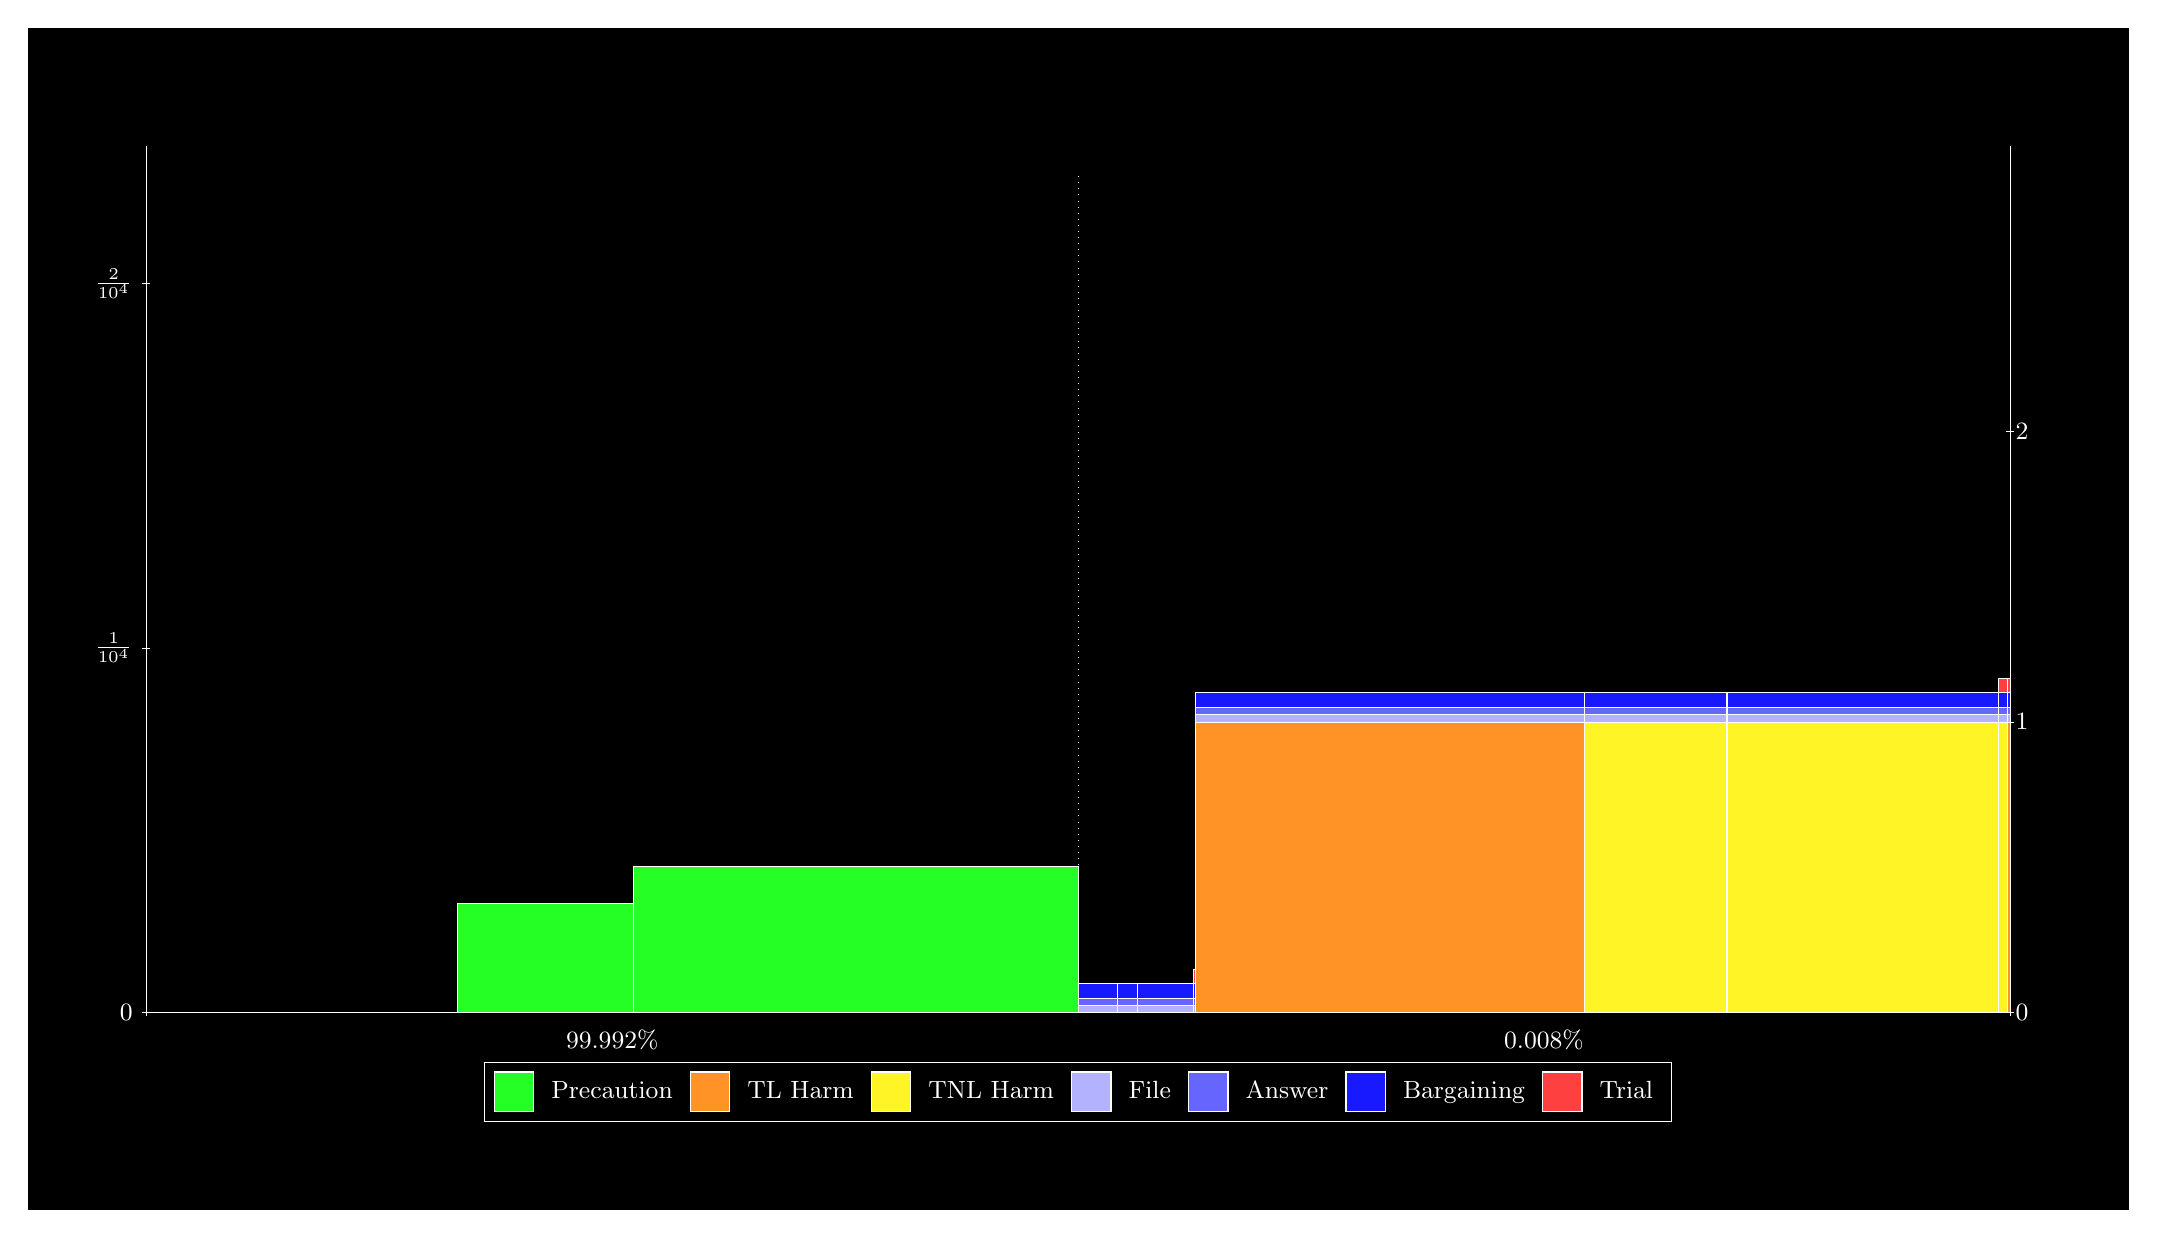
\begin{tikzpicture}
\draw[fill=black] (0,0) rectangle (26.667,15);
\draw[fill=green!85,draw=white,very thin] (5.4443,2.5) rectangle (7.6851,3.8889);
\draw[fill=green!85,draw=white,very thin] (7.6851,2.5) rectangle (13.333,4.3519);
\draw[fill=blue!30,draw=white,very thin] (13.333,2.5) rectangle (13.828,2.5923);
\draw[fill=blue!60,draw=white,very thin] (13.333,2.5923) rectangle (13.828,2.6846);
\draw[fill=blue!90,draw=white,very thin] (13.333,2.6846) rectangle (13.828,2.8692);
\draw[fill=green!85,draw=white,very thin] (13.828,2.5) rectangle (14.084,2.5001);
\draw[fill=blue!30,draw=white,very thin] (13.828,2.5001) rectangle (14.084,2.5924);
\draw[fill=blue!60,draw=white,very thin] (13.828,2.5924) rectangle (14.084,2.6847);
\draw[fill=blue!90,draw=white,very thin] (13.828,2.6847) rectangle (14.084,2.8693);
\draw[fill=green!85,draw=white,very thin] (14.084,2.5) rectangle (14.792,2.5001);
\draw[fill=blue!30,draw=white,very thin] (14.084,2.5001) rectangle (14.792,2.5924);
\draw[fill=blue!60,draw=white,very thin] (14.084,2.5924) rectangle (14.792,2.6847);
\draw[fill=blue!90,draw=white,very thin] (14.084,2.6847) rectangle (14.792,2.8693);
\draw[fill=green!85,draw=white,very thin] (14.792,2.5) rectangle (14.817,2.5001);
\draw[fill=blue!30,draw=white,very thin] (14.792,2.5001) rectangle (14.817,2.5924);
\draw[fill=blue!60,draw=white,very thin] (14.792,2.5924) rectangle (14.817,2.6847);
\draw[fill=blue!90,draw=white,very thin] (14.792,2.6847) rectangle (14.817,2.8693);
\draw[fill=red!75,draw=white,very thin] (14.792,2.8693) rectangle (14.817,3.0538);
\draw[fill=orange!85,draw=white,very thin] (14.817,2.5) rectangle (19.764,6.1916);
\draw[fill=blue!30,draw=white,very thin] (14.817,6.1916) rectangle (19.764,6.2839);
\draw[fill=blue!60,draw=white,very thin] (14.817,6.2839) rectangle (19.764,6.3762);
\draw[fill=blue!90,draw=white,very thin] (14.817,6.3762) rectangle (19.764,6.5608);
\draw[fill=green!85,draw=white,very thin] (19.764,2.5) rectangle (21.566,2.5001);
\draw[fill=yellow!85,draw=white,very thin] (19.764,2.5001) rectangle (21.566,6.1917);
\draw[fill=blue!30,draw=white,very thin] (19.764,6.1917) rectangle (21.566,6.284);
\draw[fill=blue!60,draw=white,very thin] (19.764,6.284) rectangle (21.566,6.3763);
\draw[fill=blue!90,draw=white,very thin] (19.764,6.3763) rectangle (21.566,6.5609);
\draw[fill=green!85,draw=white,very thin] (21.566,2.5) rectangle (21.58,2.5001);
\draw[fill=orange!85,draw=white,very thin] (21.566,2.5001) rectangle (21.58,6.1917);
\draw[fill=blue!30,draw=white,very thin] (21.566,6.1917) rectangle (21.58,6.284);
\draw[fill=blue!60,draw=white,very thin] (21.566,6.284) rectangle (21.58,6.3763);
\draw[fill=blue!90,draw=white,very thin] (21.566,6.3763) rectangle (21.58,6.5609);
\draw[fill=green!85,draw=white,very thin] (21.58,2.5) rectangle (25.015,2.5001);
\draw[fill=yellow!85,draw=white,very thin] (21.58,2.5001) rectangle (25.015,6.1917);
\draw[fill=blue!30,draw=white,very thin] (21.58,6.1917) rectangle (25.015,6.284);
\draw[fill=blue!60,draw=white,very thin] (21.58,6.284) rectangle (25.015,6.3763);
\draw[fill=blue!90,draw=white,very thin] (21.58,6.3763) rectangle (25.015,6.5609);
\draw[fill=green!85,draw=white,very thin] (25.015,2.5) rectangle (25.132,2.5001);
\draw[fill=yellow!85,draw=white,very thin] (25.015,2.5001) rectangle (25.132,6.1917);
\draw[fill=blue!30,draw=white,very thin] (25.015,6.1917) rectangle (25.132,6.284);
\draw[fill=blue!60,draw=white,very thin] (25.015,6.284) rectangle (25.132,6.3763);
\draw[fill=blue!90,draw=white,very thin] (25.015,6.3763) rectangle (25.132,6.5609);
\draw[fill=red!75,draw=white,very thin] (25.015,6.5609) rectangle (25.132,6.7454);
\draw[fill=green!85,draw=white,very thin] (25.132,2.5) rectangle (25.167,2.5001);
\draw[fill=orange!85,draw=white,very thin] (25.132,2.5001) rectangle (25.167,6.1917);
\draw[fill=blue!30,draw=white,very thin] (25.132,6.1917) rectangle (25.167,6.284);
\draw[fill=blue!60,draw=white,very thin] (25.132,6.284) rectangle (25.167,6.3763);
\draw[fill=blue!90,draw=white,very thin] (25.132,6.3763) rectangle (25.167,6.5609);
\draw[fill=red!75,draw=white,very thin] (25.132,6.5609) rectangle (25.167,6.7454);
\draw[white,very thin] (1.5,2.5) -- (1.5,13.5);
\draw[white,very thin] (1.45,2.5) -- (1.55,2.5);
\node[font=\small,text=white, anchor=east] at (1.45, 2.5) {0};
\draw[white,very thin] (1.45,7.1296) -- (1.55,7.1296);
\node[font=\small,text=white, anchor=east] at (1.45, 7.1296) {$\frac{1}{10^{4}}$};
\draw[white,very thin] (1.45,11.759) -- (1.55,11.759);
\node[font=\small,text=white, anchor=east] at (1.45, 11.759) {$\frac{2}{10^{4}}$};

\draw[white,dotted,very thin] (13.333,2.83) -- (13.333,13.17);
\draw[white,very thin] (25.167,2.5) -- (25.167,13.5);
\draw[white,very thin] (25.117,2.5) -- (25.217,2.5);
\node[font=\small,text=white, anchor=west] at (25.117, 2.5) {0};
\draw[white,very thin] (25.117,6.1916) -- (25.217,6.1916);
\node[font=\small,text=white, anchor=west] at (25.117, 6.1916) {1};
\draw[white,very thin] (25.117,9.8832) -- (25.217,9.8832);
\node[font=\small,text=white, anchor=west] at (25.117, 9.8832) {2};

\draw[white,very thin] (1.5,2.5) -- (25.167,2.5);
\draw[white,very thin] (1.5,2.45) -- (1.5,2.55);
\node[font=\small,text=white, anchor=north] at (1.5, 2.45) {};
\draw[white,very thin] (25.167,2.45) -- (25.167,2.55);
\node[font=\small,text=white, anchor=north] at (25.167, 2.45) {};

\node[font=\small,text=white,anchor=south] at (7.4167, 1.9) {99.992\%};
\node[font=\small,text=white,anchor=south] at (19.25, 1.9) {0.008\%};
\draw (13.3333,2.5) node (B) {};
\begin{scope}[align=center]
\matrix[scale=0.5,draw=white,below=0.5cm of B,nodes={draw},column sep=0.1cm]{
\node[rectangle,draw,minimum width=0.5cm,minimum height=0.5cm,fill=green!85]{}; & \node[draw=none,font=\small,text=white]{Precaution}; &
\node[rectangle,draw,minimum width=0.5cm,minimum height=0.5cm,fill=orange!85]{}; & \node[draw=none,font=\small,text=white]{TL Harm}; &
\node[rectangle,draw,minimum width=0.5cm,minimum height=0.5cm,fill=yellow!85]{}; & \node[draw=none,font=\small,text=white]{TNL Harm}; &
\node[rectangle,draw,minimum width=0.5cm,minimum height=0.5cm,fill=blue!30]{}; & \node[draw=none,font=\small,text=white]{File}; &
\node[rectangle,draw,minimum width=0.5cm,minimum height=0.5cm,fill=blue!60]{}; & \node[draw=none,font=\small,text=white]{Answer}; &
\node[rectangle,draw,minimum width=0.5cm,minimum height=0.5cm,fill=blue!90]{}; & \node[draw=none,font=\small,text=white]{Bargaining}; &
\node[rectangle,draw,minimum width=0.5cm,minimum height=0.5cm,fill=red!75]{}; & \node[draw=none,font=\small,text=white]{Trial}; \\\\
};\end{scope}

\end{tikzpicture}
\end{document}